<<Соединение точек>>~--- это игра для одного игрока. Игровое поле строится следующим
образом. Выбираются два целых числа, каждое из которых больше 2, которые обозначаются
$g$ и $r$. Затем на плоскости рисуются четыре точки в вершинах квадрата, две верхние из них становятся зелеными точками, а две нижние~--- красными. Далее внутри квадрата рисуются зеленые и красные точки таким образом, что никакие три точки, включая вершины квадрата, не лежат на одной прямой. Процесс продолжается до тех пор, пока общее количество зеленых точек не станет равным $g$, а количество красных точек~--- равным $r$.

После того, как игровое поле нарисовано, игрок начинает соединять точки. Две точки можно соединять отрезком, соблюдая следующие условия:
\begin{itemize}
\item соединяются только две точки одного цвета;
\item отрезок, соединяющий точки, не пересекает никакой из ранее нарисованных отрезков
(кроме как по концам отрезков).
\end{itemize}

Будем считать, что две точки $u$ и $v$ принадлежат одной компоненте, если от $u$ до $v$ можно дойти по нарисованным отрезкам.

Цель игры~--- соединить все зеленые точки в одну компоненту с помощью $g - 1$ отрезков, а все красные точки~--- в другую компоненту с помощью $r - 1$ отрезков. Можно доказать, что при вышеописанном способе расположения точек всегда существует способ выиграть игру. 

Вам будет задано квадратное игровое поле со стороной $s$, а также $g$ зелеными и $r$ красными точками. Координаты точек задаются парами целых чисел $(x_i, y_i)$. Зеленые точки пронумерованы числами от $1$ до $g$ так, что верхняя левая точка $(0, s)$ имеет номер 1, верхняя правая точка $(s, s)$~--- номер 2, а остальные точки~--- номера от $3$ до $g$ (в произвольном порядке). Красные точки пронумерованы числами от $1$ до $r$ так, что нижняя левая точка $(0, 0)$ имеет номер 1, нижняя правая точка $(s, 0)$~--- номер 2, а остальные точки~--- номера от $3$ до $r$ (в произвольном порядке).

Напишите программу, которая по заданным координатам $g$ зеленых точек и координатам r
красных точек находит способ, как нарисовать $g - 1$ зеленых отрезков и $r - 1$ красных отрезков таким образом, чтобы все зеленые точки принадлежали одной компоненте, а все красные точки~--- другой, и никакие два отрезка не пересекались.

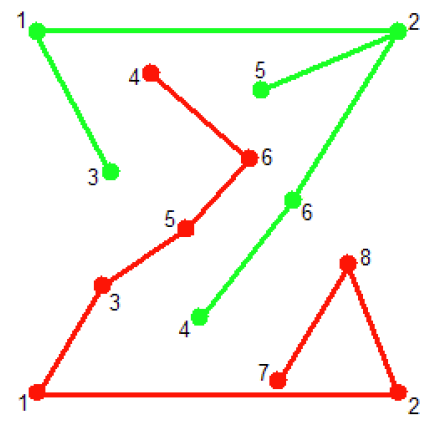
\includegraphics{points.png}

На рисунке показан пример игры, где зеленые точки соединены в одну компоненту, а красные точки~--- в другую. Легко видеть, что никакие три точки на рисунке не
лежат на одной прямой, и никакие два отрезка не пересекаются, кроме как по концам.

Напишите программу, которая по заданным координатам $g$ зеленых точек и координатам $r$
красных точек находит способ, как нарисовать $(g - 1)$ зеленых отрезков и $(r - 1)$ красных отрезков таким образом, чтобы все зеленые точки принадлежали одной компоненте, а все красные точки~--- другой, и никакие два отрезка не пересекались.